% \documentclass[10pt]{beamer}
  \documentclass[9pt]{beamer}
% \usetheme{Boadilla}
% \usetheme{default}
% \useoutertheme{infolines}
  \usetheme[numbering=counter]{metropolis}
  \definecolor{lightgray}{gray}{0.9}
% \definecolor{test1}{RGB}{250, 250, 230}
  \definecolor{test1}{RGB}{255, 255, 235}
  \definecolor{test2}{RGB}{240, 240, 250}
% \setbeamercolor{frametitle}{fg=black,bg=white}
  \setbeamercolor{frametitle}{fg=black,bg=test1}
  \setbeamercolor{background canvas}{bg=test2}
  \setbeamertemplate{frame footer}{UMBC Atmospheric Spectroscopy Lab}


% acronyms for text or math mode
% \newcommand {\ccast} {\mbox{\small\textsc{ccast}}}
\newcommand {\ccast} {\mbox{\small CCAST}}
\newcommand {\nedn} {\mbox{\small NEdN}}
\newcommand {\kcarta} {\mbox{k\small{CARTA}}}

\newcommand {\chirp} {\mbox{\small CHIRP}}
\newcommand {\cris}  {\mbox{\small CrIS}}
\newcommand {\airs}  {\mbox{\small AIRS}}
\newcommand {\iasi}  {\mbox{\small IASI}}
\newcommand {\idps}  {\mbox{\small IDPS}}
\newcommand {\nasa}  {\mbox{\small NASA}}
\newcommand {\noaa}  {\mbox{\small NOAA}}
\newcommand {\nstar} {\mbox{\small STAR}}
\newcommand {\umbc}  {\mbox{\small UMBC}}
\newcommand {\uw}    {\mbox{\small UW}}

\newcommand {\fft}  {\mbox{\small FFT}}
\newcommand {\ifft} {\mbox{\small IFFT}}
\newcommand {\fir}  {\mbox{\small FIR}}
\newcommand {\fov}  {\mbox{\small FOV}}
\newcommand {\for}  {\mbox{\small FOR}}
\newcommand {\ict}  {\mbox{\small ICT}}
\newcommand {\ils}  {\mbox{\small ILS}}
\newcommand {\igm}  {\mbox{\small IGM}}
\newcommand {\opd}  {\mbox{\small OPD}}
\newcommand {\rms}  {\mbox{\small RMS}}
\newcommand {\zpd}  {\mbox{\small ZPD}}
\newcommand {\ppm}  {\mbox{\small PPM}}
\newcommand {\srf}  {\mbox{\small SRF}}
\newcommand {\sdr}  {\mbox{\small SDR}}
\newcommand {\FWHM} {\mbox{\small FWHM}}
\newcommand {\fwhm} {\mbox{\small\textsc{fwhm}}}

\newcommand {\ES} {\mbox{\small ES}}
\newcommand {\SP} {\mbox{\small SP}}
\newcommand {\IT} {\mbox{\small IT}}
\newcommand {\SA} {\mbox{\small SA}}

\newcommand {\ET} {\mbox{\small ET}}
\newcommand {\FT} {\mbox{\small FT}}

\newcommand {\wn} {\mbox{cm$^{-1}$}}
\newcommand {\cm} {\mbox{cm}}

% abbreviations, mainly for math mode
\newcommand {\real} {\mbox{real}}
\newcommand {\imag} {\mbox{imag}}
\newcommand {\atan} {\mbox{atan}}
\newcommand {\obs}  {\mbox{obs}}
\newcommand {\calc} {\mbox{calc}}
\newcommand {\sinc} {\mbox{sinc}}
\newcommand {\psinc} {\mbox{psinc}}
\newcommand {\std} {\mbox{std}}
\newcommand {\nchan} {\mbox{nchan}}
\newcommand {\nobs} {\mbox{nobs}}

% symbols, for math mode only
\newcommand {\lmax} {L_{\mbox{\tiny max}}}
\newcommand {\vmax} {V_{\mbox{\tiny max}}}

\newcommand {\tauobs} {\tau_{\mbox{\tiny obs}}}
\newcommand {\taucal} {\tau_{\mbox{\tiny calc}}}
\newcommand {\Vdc}  {V_{\mbox{\tiny DC}}}

\newcommand {\rIT} {r_{\mbox{\tiny\textsc{ict}}}}
\newcommand {\rES} {r_{\mbox{\tiny\textsc{es}}}}
\newcommand {\robs} {r_{\mbox{\tiny obs}}}

\newcommand {\rITobs} {r_{\mbox{\tiny\textsc{ict}}}^{\mbox{\tiny obs}}}
\newcommand {\rITcal} {r_{\mbox{\tiny\textsc{ict}}}^{\mbox{\tiny cal}}}

\newcommand {\rESuser} {r_{\mbox{\tiny\textsc{es}}}^{\mbox{\tiny user}}}
\newcommand {\rITuser} {r_{\mbox{\tiny\textsc{ict}}}^{\mbox{\tiny user}}}
\newcommand {\rITsensor} {r_{\mbox{\tiny\textsc{ict}}}^{\mbox{\tiny sensor}}}
\newcommand {\rITfov} {r_{\mbox{\tiny\textsc{ict}}}^{\mbox{\tiny fov}}}

\newcommand {\fcos} {f_{\mbox{\tiny cos}}}
\newcommand {\fatbd} {f_{\mbox{\tiny\textsc{atbd}}}}

\newcommand {\ITmean} {\langle\mbox{\small IT}\rangle}
\newcommand {\SPmean} {\langle\mbox{\small SP}\rangle}

\newcommand {\Ttc} {t^{\mbox{\tiny\textsc{tc}}}}
\newcommand {\Tac} {t^{\mbox{\tiny\textsc{ac}}}}
\newcommand {\rtc} {r_{\mbox{\tiny\textsc{tc}}}}
\newcommand {\rta} {r_{\mbox{\tiny\textsc{ta}}}}



\title{
  Implementation and Overview \\
  of the CHIRP Radiance Product \\
}
\author{H.~E.~Motteler and L.~L.~Strow}

\institute{
  UMBC Atmospheric Spectroscopy Lab \\
  Joint Center for Earth Systems Technology \\
}
\date{\today}
\begin{document}

%----------- slide --------------------------------------------------%
\begin{frame}[plain]
\titlepage
\end{frame}
%----------- slide --------------------------------------------------%
\begin{frame}
\frametitle{Introduction}
\begin{itemize}

  \item {\chirp} is the translation of {\cris} L1b and {\airs} L1c files 
    to a common, more generic L1c format.  We present an overview of the
    translation and format.  Topics include:

  \begin{itemize}
    \item The {\chirp} translations
    \item The {\chirp} L1c data format
    \item {\airs}-parent QC and NEdN
    \item {\cris}-parent QC and NEdN
%   \item {\airs} and {\cris} sampling
%   \item {\airs} translation residuals
  \end{itemize}

  \item We have been doing {\airs}-to-{\cris} translations for
    several years now, mainly for analyzing SNOs.  {\chirp} is
    a continuation of that work.

  \item We plan to do {\chirp} translations for {\airs}, {\cris}
    SNPP, {\cris} J1, and (going forward) J2--J4, with a schedule to
    be determined for crossover times, to produce a single long-term
    climate record.

  \item {\chirp} will be released soon by the JPL Sounder SIPS as a
    product at the GSFC-DIS.

\end{itemize}
\end{frame}
%----------- slide --------------------------------------------------%
\begin{frame}
\frametitle{Sample AIRS and AIRS-parent CHIRP}
\begin{columns}[t]
\begin{column}{0.5\textwidth}  
  \begin{centering}
  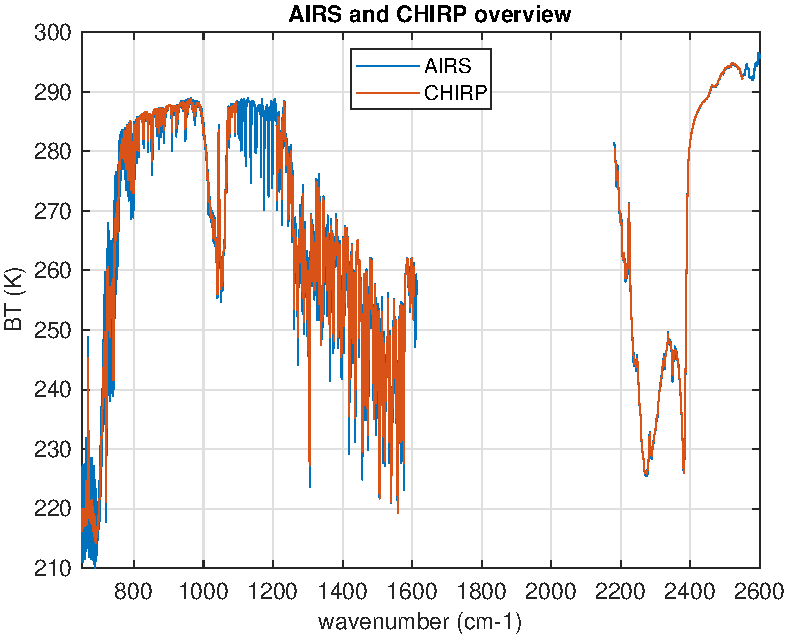
\includegraphics[width=\textwidth]{figures/airs_and_chirp_overview.pdf}
  \end{centering}\vspace{3mm}

Sample {\airs} and {\airs}-parent {\chirp} spectra, granule means
for 19 Aug 2018 granule 25.  The {\chirp} bands are the intersection
of the {\airs} and {\cris} bands.

\end{column}

\begin{column}{0.5\textwidth}
  \begin{centering}
  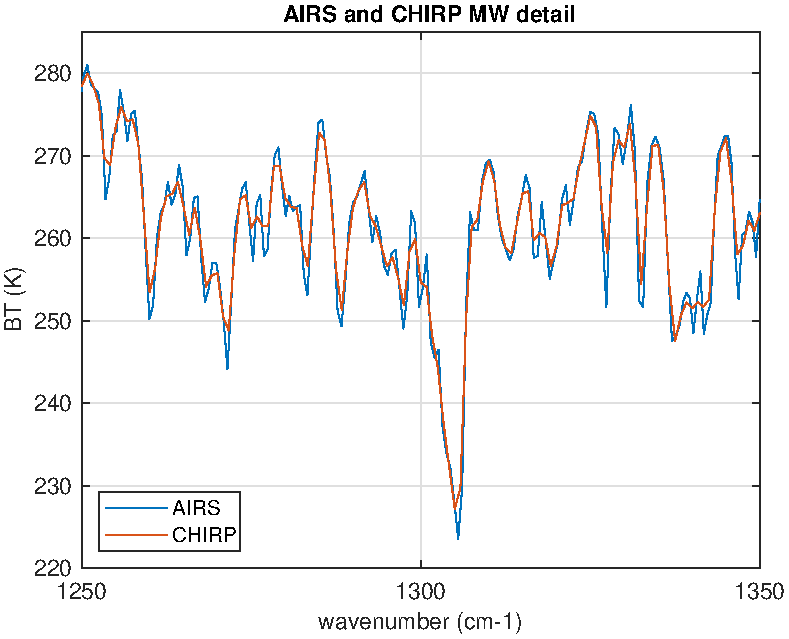
\includegraphics[width=\textwidth]{figures/airs_and_chirp_mw_detail.pdf}
  \end{centering}\vspace{3mm}

MW detail from the same granule.  Note that the data are on two
different grids, and what we mainly see is the effect of the {\chirp}
apodization.

\end{column}
\end{columns}
\end{frame}
%----------- slide --------------------------------------------------%
\begin{frame}
\frametitle{The Translations}

\begin{itemize}

  \item For the {\airs} to {\chirp} translation, we deconvolve
    {\airs} to an intermediate grid, typically $0.1$ {\wn}, with a
    Moore-Penrose pseudo-inverse of tabulated {\airs} SRFs, and then
    reconvolve to the {\cris} ``mid res'' (aka \chirp) user grid via
    resampling or double Fourier interpolation.

  \item This is described in detail in ``{\airs} deconvolution and
    the translation of {\airs}-to-{\cris} radiances with applications
    for the IR climate record,'' IEEE Transactions on Geoscience and
    Remote Sensing, 57(3):1793--1803, 2018.

  \item The {\cris} to {\chirp} translation is done by interpolation
    from the {\cris} high res product (0.8/0.8/0.8 cm \opd).  {\chirp}
    can also be produced directly by {\umbc} {\ccast} ({\cris} L0 to
    L1b processing), with a single interpolation from the sensor to
    the {\chirp} user grid.

  \item Hamming apodization and an optional bias correction are
    applied to both translations.  Currently {\airs} and {\cris} J1
    parent are adjusted to match {\cris} SNPP.

\end{itemize}
\end{frame}
%----------- slide --------------------------------------------------%
\begin{frame}
\frametitle{CHIRP sample ILS}
\begin{center}
  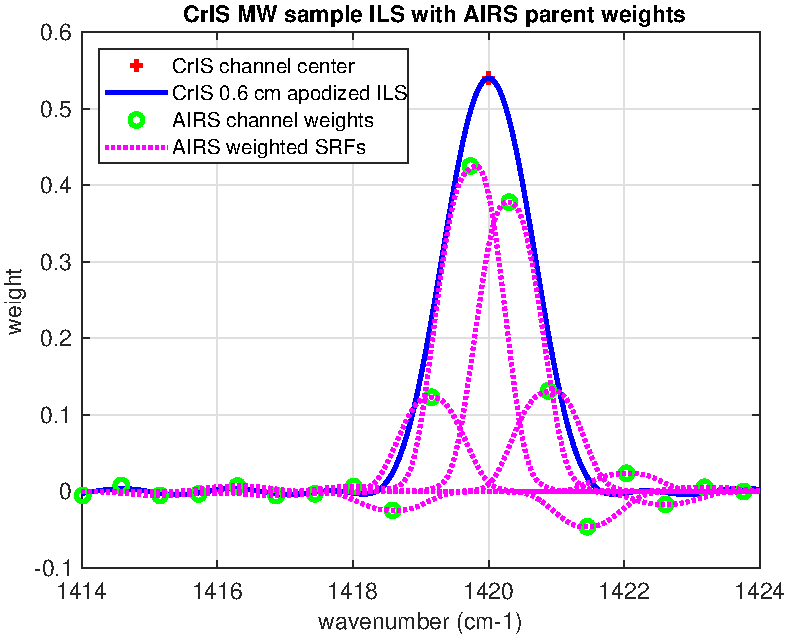
\includegraphics[scale=0.5]{figures/sample_CrIS_ILS_with_AIRS_parent_SRFs.pdf}
\end{center}
\vspace{-3mm}

The MW {\chirp} apodized ILS, together with weights for the {\airs}
channels, \\ for the {\cris} or {\chirp} channel shown.  The {\airs}
weights are paired with the corresponding AIRS SRFs, normalized to
the weight values.

% (The weights are from a row of a linearized approximation of the
% {\airs} to {\cris} translation.)

\end{frame} % source a2cris_srfs.m
%----------- slide --------------------------------------------------%
\begin{frame}
\frametitle{CHIRP Data Format}
\begin{itemize}

  \item {\chirp} radiances are for a nominal 3-band interferometer 
    with an {\opd} of $0.8$ {\cm} in the long-wave (LW), $0.6$ {\cm}
    in the medium-wave (MW), and $0.4$ {\cm} in the short-wave (SW)
    bands.

  \item The {\chirp} ILS is the Hamming-apodized sinc ILS for $0.8$
    {\cm} (LW), $0.6$ {\cm} (MW), and $0.4$ {\cm} (SW) {\opd}s, and is
    the same for the {\airs} and {\cris} parent data.

  \item After translation from {\cris} the three bands have 713, 649,
    and 317, channels, respectively.  These are concatenated for the
    {\chirp} product, for a total of 1679 channels.

  \item {\airs}-parent {\chirp} uses the same channel set.  However
    the {\airs}-to-{\cris} ``midres'' translation we use for {\chirp}
    gives only 1483 channels, due to slightly different band spans.
    These are embedded in the 1679 channel set, with missing channels
    flagged.

\end{itemize}
\end{frame}
%----------- slide --------------------------------------------------%
\begin{frame}
\frametitle{CHIRP Data Format}
\begin{itemize}

  \item {\chirp} granules correspond with their parent {\airs} or
    {\cris} granules, \\ and inherit most of the parent granule's
    attributes and supporting data.

  \item {\cris} L1b radiance data is organized as an $\nchan_1
    \times 9 \times 30 \times 45$ $=\nchan_1 \times 12150$ array,
    channels by FOVs by cross-track index by along-track index.

  \item {\airs} L1c radiance data is organized as an $\nchan_2
    \times 90 \times 135$ $= \nchan_2 \times 12150$ array, channels
    by cross-track index by along-track index.
  
  \item {\chirp} radiance data is reshaped to a $1679 \times 12150$
    array, channels by observation, in time order.  Each ``obs'' has
    an associated values for time, {\fov} (for {\cris}), original
    indices for {\airs} or {\cris}, along with most of the geo,
    support data, and product attributes from the parent sounders.

  \item {\chirp} granules follow JPL conventions for field names and
    attributes, and are saved in netCDF.

\end{itemize}
\end{frame}
%----------- slide --------------------------------------------------%
\begin{frame}
\frametitle{AIRS-parent CHIRP QC}

\begin{itemize}

  \item We create two QC fields per granule, rad\_qc, a 12150-vector
    with one flag value per obs, and chan\_qc, a 1679-vector with one
    flag value per channel.  For both, 0 = OK, 1 = warn, and 2 = bad.
    rad\_qc is always 0 or 2, because {\airs} L1c doesn't have a ``warn''
    flag.

  \item rad\_qc is set as a combination of the {\airs} L1c field
    instrument\_state and sanity checks on radiance and geo values.

  \item chan\_qc is set to ``bad'' for those channels in the larger
    {\chirp} 1679- channel set that are not part of the 1483 channel
    set translated from {\airs}.

  \item chan\_qc is set to ``warn'' for the 6 channels at band edges.

\end{itemize}
\end{frame}
%----------- slide --------------------------------------------------%
\begin{frame}
\frametitle{AIRS-parent CHIRP QC}

\begin{itemize}

  \item As an alternative to ``warn'' and to fill band gaps, {\airs}
    L1c provides synthetic values for some channels.  These are
    flagged individually in the L1c file, and in addition there is a
    per-granule summary, L1cNumSynth, for each channel.

  \item We linearize the {\airs} to {\cris} translation and apply
    this to the {\airs} values to get corresponding NumSynth values
    for {\chirp}.  These are normalized as a fraction and becomes
    the {\chirp} field synth\_frac.

  \item Then if $\hbox{synth\_frac} > 0.25$, we set chan\_qc to
    ``warn''.  The threshold $0.25$ is a parameter that can be changed
    in the production YAML specs.

  \item The following slides show the distribution of synthetic
    values from 20 days of {\airs} data, and analogous values for
    synth\_frac from a representative {\chirp} granule.

\end{itemize}
\end{frame}
%----------- slide --------------------------------------------------%
\begin{frame}
\frametitle{AIRS L1c Synthetic Channels}
\begin{columns}[t]
\begin{column}{0.5\textwidth}  
  \begin{centering}
  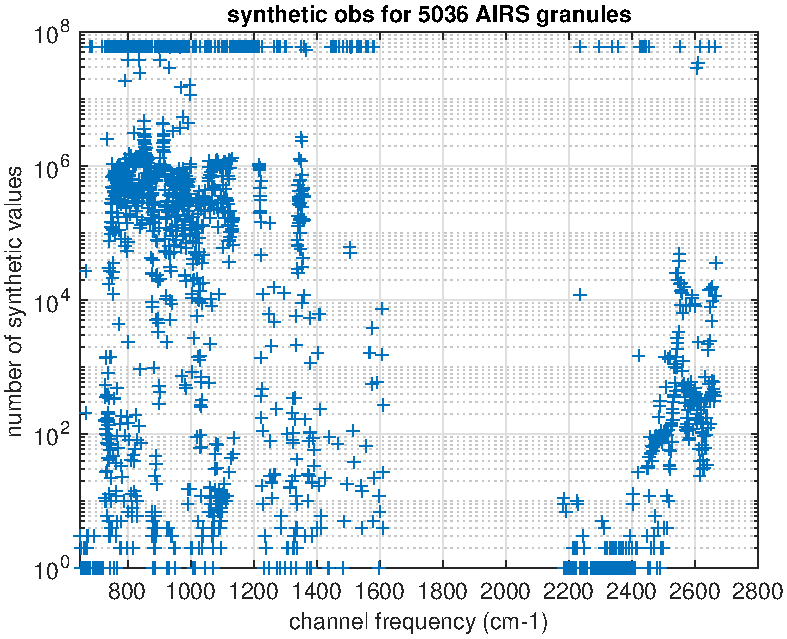
\includegraphics[width=\textwidth]{figures/synth_obs_freq_order.pdf}
  \end{centering}\vspace{3mm}

The sum of synthetic obs by channel for 5036 {\airs} granules.
Counts are on a log scale.

\end{column}

\begin{column}{0.5\textwidth}
  \begin{centering}
  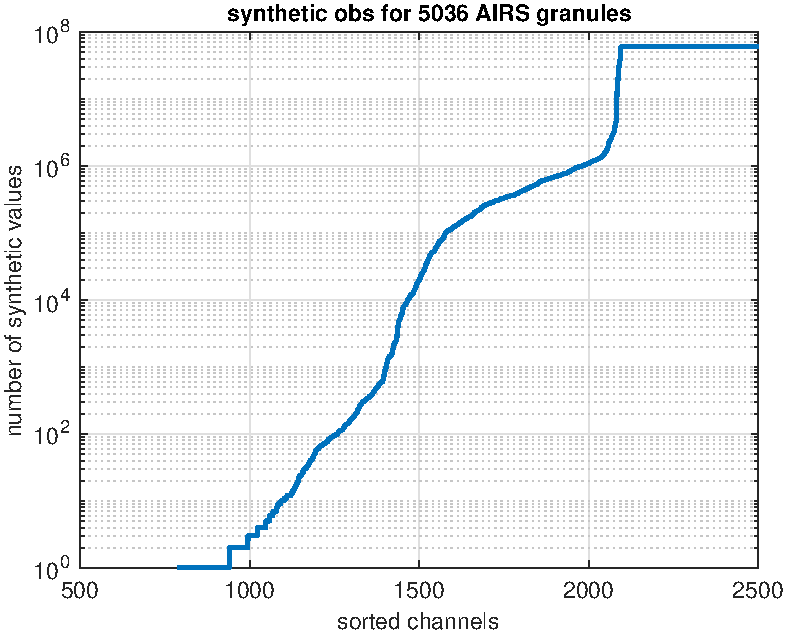
\includegraphics[width=\textwidth]{figures/synthetic_obs_counts.pdf}
  \end{centering}\vspace{3mm}

Synthetic obs per channel, sorted by number of synthetic obs.  This
shows the range of values.

\end{column}
\end{columns}
\end{frame}
%----------- slide --------------------------------------------------%
\begin{frame}
\frametitle{CHIRP sample granule synth\_frac values}
\begin{columns}[t]
\begin{column}{0.5\textwidth}  
  \begin{centering}
  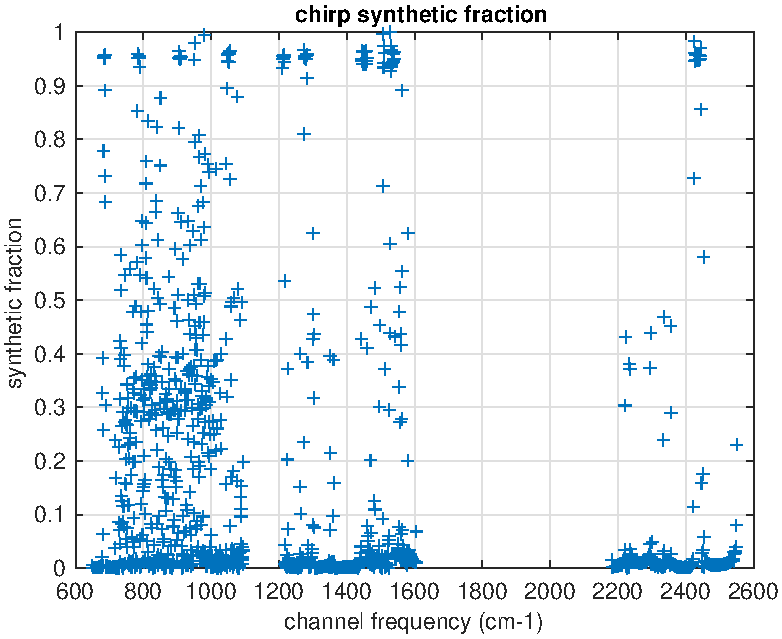
\includegraphics[width=\textwidth]{figures/chirp_sample_syn_frac.pdf}
  \end{centering}\vspace{3mm}

{\airs}-parent {\chirp} synthetic fraction for a single representative
granule.  This can be used to select channels with a relatively small
synthetic component.

\end{column}

\begin{column}{0.5\textwidth}
  \begin{centering}
  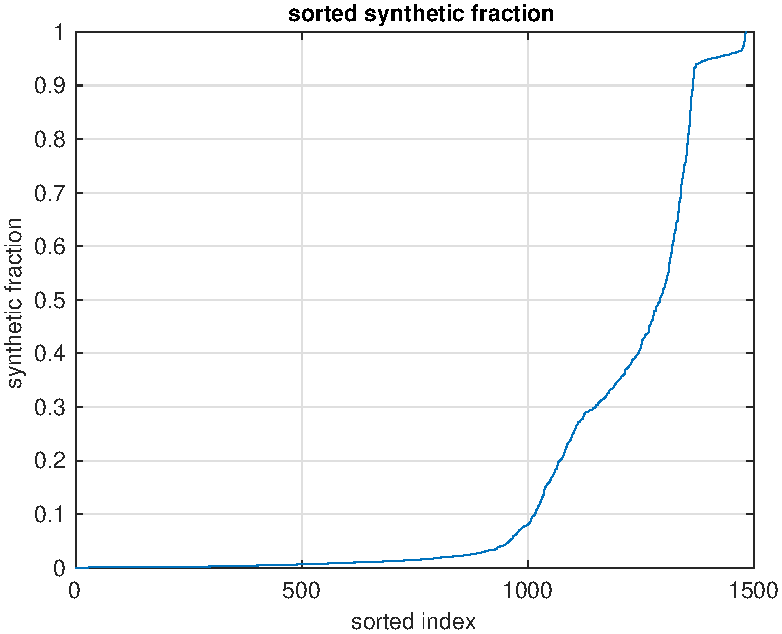
\includegraphics[width=\textwidth]{figures/chirp_sorted_syn_frac.pdf}
  \end{centering}\vspace{3mm}

{\airs}-parent {\chirp} synthetic fraction, sorted by synthetic
fraction magnitude.  This shows the variability of synth\_frac.

\end{column}
\end{columns}
\end{frame}
%----------- slide --------------------------------------------------%
\begin{frame}
\frametitle{AIRS-parent CHIRP NEdN}

\begin{itemize}

  \item {\nedn} for {\airs}-parent {\chirp} is estimated by adding
    simulated {\airs} noise at 280K, doing the translation, and
    measuring the resulting noise.  This is done repeatedly and the
    mean of the measurement is reported.

  \item To get the {\airs} estimate, we take the mean of valid
    {\nedn} values over an {\airs} granule, and interpolate over
    gaps from the synthetic channels.  {\airs} L1c does not provide
    an {\nedn} estimate for these channels, so perhaps this is the
    best we can do.

  \item More detail on the noise estimate is provided in the IEEE TGRS
    {\airs} deconvolution paper, mentioned above.

  \item The correlated fraction of {\airs} noise varies from module
    to module, and is significant for some modules.  The translation
    will preserve this correlation.  {\nedn} estimates for such
    cases are a matter for future work.

\end{itemize}
\end{frame}
%----------- slide --------------------------------------------------%
\begin{frame}
\frametitle{AIRS and CrIS parent CHIRP NEdN}
\begin{columns}[t]
\begin{column}{0.5\textwidth}  
  \begin{centering}
  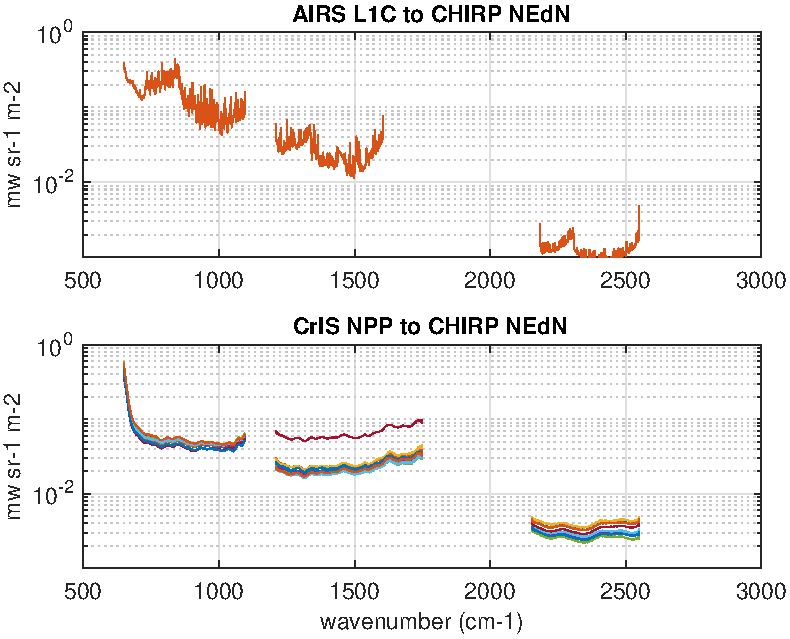
\includegraphics[width=\textwidth]{figures/chirp_nedn_from_airs_and_cris.pdf}
  \end{centering}\vspace{3mm}

Sample {\chirp} {\nedn} for {\airs} and {\cris} parent data, 2018 doy
231 granules 25 and 21, two relatively warm granules.

\end{column}

\begin{column}{0.5\textwidth}
  \begin{centering}
  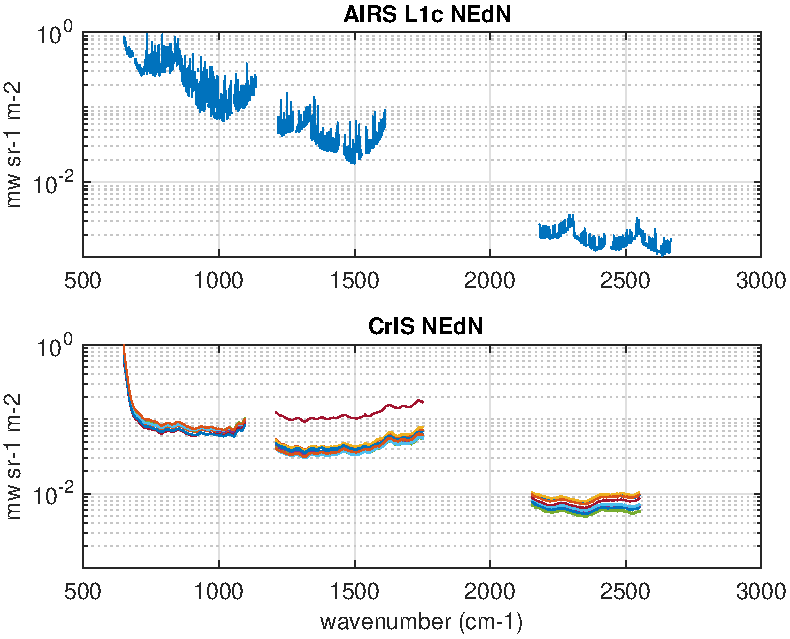
\includegraphics[width=\textwidth]{figures/sample_airs_and_cris_nedn.pdf}
  \end{centering}\vspace{3mm}

Sample {\airs} and {\cris} {\nedn} for the same two granules, 2018 doy
231 granules 25 and 21.

\end{column}
\end{columns}
\end{frame}
%----------- slide --------------------------------------------------%
\begin{frame}
\frametitle{CrIS-parent CHIRP NEdN and QC}

\begin{itemize}

  \item In comparison with {\airs}, estimating {\cris}-parent
    {\chirp} {\nedn} and doing QC is relatively simple.

  \item {\cris}-parent {\chirp} {\nedn} is derived from the high
    res {\cris} {\nedn} with scale factors to take into account the
    interpolation and apodization.  These are
    \begin{itemize}
      \item LW, 0.6325, for Hamming apodization only
      \item MW, 0.5455, for interpolation and Hamming apodization
      \item SW, 0.4446, for interpolation and Hamming apodization
    \end{itemize}

  \item {\cris}-parent {\chirp} QC is determined from the {\cris}
    parent, by combining the fields for the individual {\cris} bands.

  \item chan\_qc is set to 0 (OK) for {\cris}-parent {\chirp}.

  \item possibly we should set chan\_qc to ``warn'' at the band
    edges, as we do for {\airs} parent, but we are not doing this
    now.

\end{itemize}
\end{frame}
%----------- slide --------------------------------------------------%
\begin{frame}
\frametitle{Conclusions and Future Work}
\begin{itemize}

  \item This talk can serve as a draft for a significant part of the
    {\chirp} User's guide.

  \item Future work includes refining bias vectors and taking
    account of {\airs} correlations in the {\nedn} estimates.

  \item Closely related work includes future gridded products, which
    share many parts with the {\chirp} L1c processing.


\end{itemize}
\end{frame}
%----------- slide --------------------------------------------------%

\end{document}

